%----------------------------------------------------------------------------------------
%  A1 portrait poster: Implementing Conditional Access on FPGA
%  Compile with pdfLaTeX. logo.png sits next to this file.
%  Figures: figures/make_figs.py (uaf_steps, problem_with) and figures/make_figs_v3.py
%  (everything else); repo_qr.png links to the repository.
%----------------------------------------------------------------------------------------

\documentclass{article}
\usepackage[paperwidth=594mm,paperheight=841mm,margin=10mm]{geometry}

\usepackage[T1]{fontenc}
\usepackage{newtxtext,newtxmath}   % Times
\usepackage{newtxtt}
\usepackage{anyfontsize}

\usepackage[dvipsnames]{xcolor}
\definecolor{navy}{HTML}{1F3A5F}
\definecolor{rulegray}{HTML}{B5B5B5}
\definecolor{captiongray}{HTML}{333333}
\definecolor{caorange}{HTML}{C8521F}
\definecolor{statbg}{HTML}{EEF3F9}

\usepackage{multicol}
\setlength{\columnsep}{10mm}
\setlength{\columnseprule}{0.6pt}
\renewcommand{\columnseprulecolor}{\color{rulegray}}

\usepackage{graphicx}
\graphicspath{{figures/}}
\usepackage{booktabs}
\usepackage{array}
\usepackage{enumitem}
\usepackage{alltt}
\usepackage[hidelinks]{hyperref}

\pagestyle{empty}
\setlength{\parindent}{0pt}
\setlength{\parskip}{4pt}

% Type scale (A1)
\newcommand{\bodysize}{\fontsize{17}{21.5}\selectfont}
\newcommand{\smallsize}{\fontsize{14}{17}\selectfont}
\newcommand{\headsize}{\fontsize{30}{36}\selectfont}

\setlist{itemsep=4pt,topsep=3pt,parsep=0pt,leftmargin=1.1em}

\newcounter{psec}
\newcommand{\psection}[1]{%
  \par\vspace{4pt}\stepcounter{psec}%
  {\headsize\bfseries\color{navy}\thepsec\hspace{0.5em}#1\par}%
  \vspace{-3pt}{\color{navy}\rule{\columnwidth}{1.2pt}}\par\vspace{-4pt}}
\newcommand{\psub}[1]{\par\vspace{3pt}{\fontsize{22}{26}\selectfont\bfseries\color{navy}#1\par}\vspace{1pt}}

\newcounter{pfig}
\newcommand{\pcaption}[1]{\stepcounter{pfig}%
  {\smallsize\color{captiongray}\textbf{Figure \thepfig.} #1\par}}
\newcommand{\posterfig}[3][1.0]{%
  \par\vspace{3pt}{\centering\includegraphics[width=#1\linewidth]{#2}\par}
  \vspace{2pt}\pcaption{#3}\vspace{1pt}}

% One-line "key result" with an arrow
\newcommand{\key}[1]{\item[\textcolor{caorange}{\large$\blacktriangleright$}] #1}

\newsavebox{\codebox}
\begin{document}
\bodysize

%----------------------------------------------------------------------------------------
%  HEADER
%----------------------------------------------------------------------------------------
\noindent
\begin{minipage}[c]{0.14\linewidth}
  \IfFileExists{logo.png}{\def\haslogo{1}}{\IfFileExists{figures/logo.png}{\def\haslogo{1}}{}}%
  \ifdefined\haslogo
    
\includegraphics[width=\linewidth,height=48mm,keepaspectratio]{logo.png}%
  \else
    \fbox{\parbox[c][44mm][c]{0.9\linewidth}{\centering [LOGO]}}%
  \fi
\end{minipage}%
\begin{minipage}[c]{0.72\linewidth}\centering
  {\fontsize{56}{64}\selectfont\bfseries\color{navy} Implementing Conditional Access on FPGA\par}
  \vspace{3mm}
  {\fontsize{26}{32}\selectfont A dual-core, cache-coherent RISC-V processor with conditional access~[1], on an AMD KR260\par}
  \vspace{2mm}
  {\fontsize{26}{32}\selectfont Aryan Kumar, Nishant Dhankhar, Kudumula Vinod Kumar Reddy\qquad\textit{Advisor:} Ajay Singh\par}
  \vspace{2mm}
  {\fontsize{22}{28}\selectfont\itshape Department of Computer Science and Engineering, IIT Gandhinagar\par}
\end{minipage}%
\begin{minipage}[c]{0.14\linewidth}\centering
  \href{https://github.com/turing-house-community/multicore-on-fpga}{
\includegraphics[height=34mm]{repo_qr.png}}\par
  \vspace{1.5mm}{\fontsize{15}{18}\selectfont\color{navy}\bfseries Code and data\par}
\end{minipage}

\vspace{3mm}
{\color{navy}\rule{\linewidth}{2pt}}
\vspace{1mm}

\begin{multicols}{2}
\raggedcolumns
\bodysize

%----------------------------------------------------------------------------------------
\psection{The problem: use-after-free}
%----------------------------------------------------------------------------------------
In a lock-free data structure, threads read shared nodes without taking locks while
other threads remove them. If a removed node is freed while another core still holds a
pointer to it, that core reads freed memory (Figure~1).

\posterfig[0.88]{uaf_steps.png}{A use-after-free on a shared linked list.}

%----------------------------------------------------------------------------------------
\psection{Existing software approaches}
%----------------------------------------------------------------------------------------
\begin{itemize}
  \item \textbf{Hazard pointers (HP)}~[3]: a reader announces each pointer before using it, and
        a node is freed only when no announcement names it. \emph{Problem:} every read pays a
        memory fence, which slows traversals.
  \item \textbf{Epoch-based reclamation (EBR)}~[4]: removed nodes are freed in batches once every
        thread has passed a quiescent point. \emph{Problem:} unfreed memory piles up, without
        bound if one thread stalls.
\end{itemize}
\textbf{The common issue: delayed reclamation.} Both schemes free a node only some time
after it is removed, so they trade speed against memory.

%----------------------------------------------------------------------------------------
\psection{Solution: Conditional Access}
%----------------------------------------------------------------------------------------
Conditional Access (CA)~[1] adds memory instructions that \emph{watch} the cache lines a
thread reads. If another core writes one, the thread's next CA instruction \emph{fails}
and it retries. So a removed node can be freed \textbf{immediately}.

\noindent
\begin{minipage}[c]{0.44\linewidth}
  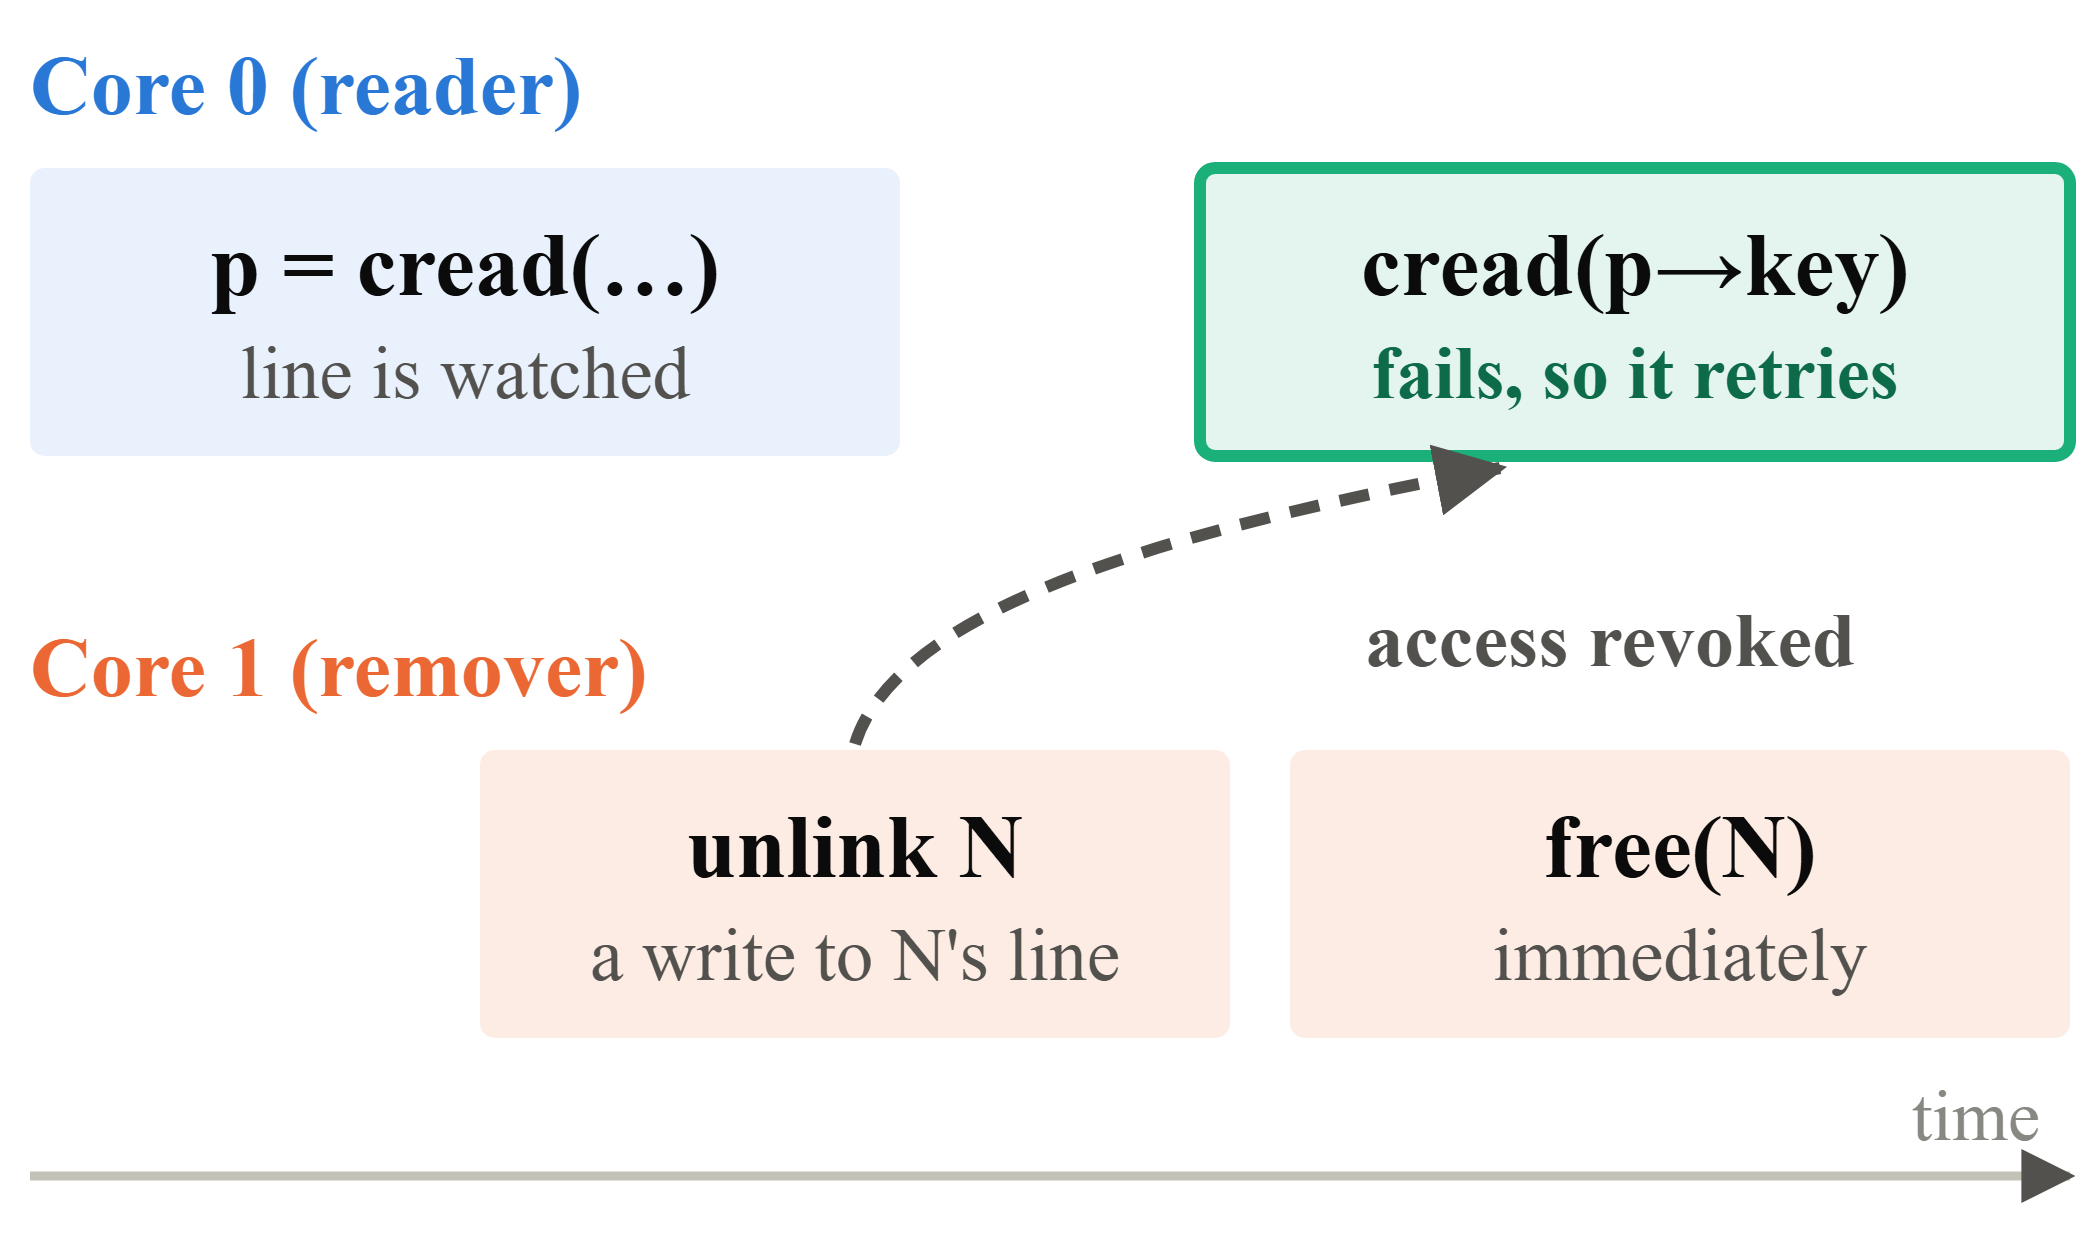
\includegraphics[width=\linewidth]{problem_with.png}
\end{minipage}\hfill
\begin{minipage}[c]{0.53\linewidth}
  \pcaption{The remover's write revokes the reader's access, so the reader retries
  instead of using freed memory.}
  \vspace{6pt}
  {\smallsize\itshape The four instructions of~[1], which we built in hardware, and the one we added:\par}
  \vspace{3pt}
  \begin{tabular}{@{}ll@{}}
    \texttt{cread}    & load and watch the line\\
    \texttt{cwrite}   & store if nothing watched changed\\
    \texttt{untagOne} & stop watching one line\\
    \texttt{untagAll} & stop watching all lines\\
    \textcolor{caorange}{\texttt{bcafail}} & \textcolor{caorange}{jump if a CA op failed}\\
  \end{tabular}
\end{minipage}


\psub{What the software looks like}
\begin{lrbox}{\codebox}\begin{minipage}{\dimexpr\columnwidth-2\fboxsep\relax}
\fontsize{14}{16.5}\selectfont
\begin{alltt}
\textbf{void} pop(\textbf{void}) \{                  \textcolor{captiongray}{// from our stack benchmark}
retry: untagAll();
  node *t  = cread(\&top);         \textcolor{captiongray}{// read top and watch its line}
  \textbf{if} (bcafail()) \textbf{goto} retry;      \textcolor{caorange}{// one branch: did a watched line change?}
  node *nx = cread(\&t->next);     \textcolor{captiongray}{// watch t as well}
  \textbf{if} (bcafail()) \textbf{goto} retry;
  cwrite(\&top, nx);               \textcolor{captiongray}{// store only if top and t are unchanged}
  \textbf{if} (bcafail()) \textbf{goto} retry;
  untagAll(); free(t);            \textcolor{caorange}{// safe at once: any reader of t will fail}
\}
\end{alltt}
\vspace{-14pt}
\end{minipage}\end{lrbox}
\noindent\colorbox{statbg}{\usebox{\codebox}}\par
\stepcounter{pfig}{\smallsize\color{captiongray}\textbf{Figure \thepfig.} A stack pop with CA
(simplified): no hazard pointers or epochs, the node is freed as soon as it is unlinked.\par}

\psection{System design, on a real FPGA}
%----------------------------------------------------------------------------------------
CA was only ever evaluated in a simulator. Real hardware answers: \textbf{does it work}, \textbf{what
does it cost}, and \textbf{can a simulator be trusted?} Starting from CVA6~[2], an open-source
single-core RISC-V processor, we added
\textbf{(1)} a second core, \textbf{(2)} MSI cache coherence through a directory,
\textbf{(3)} the CA instructions plus \texttt{bcafail}, and \textbf{(4)} a shared L2 cache,
as in~[1].

\vspace{4pt}\noindent\colorbox{statbg}{\begin{minipage}{\dimexpr\columnwidth-2\fboxsep\relax}
  \vspace{4pt}{\centering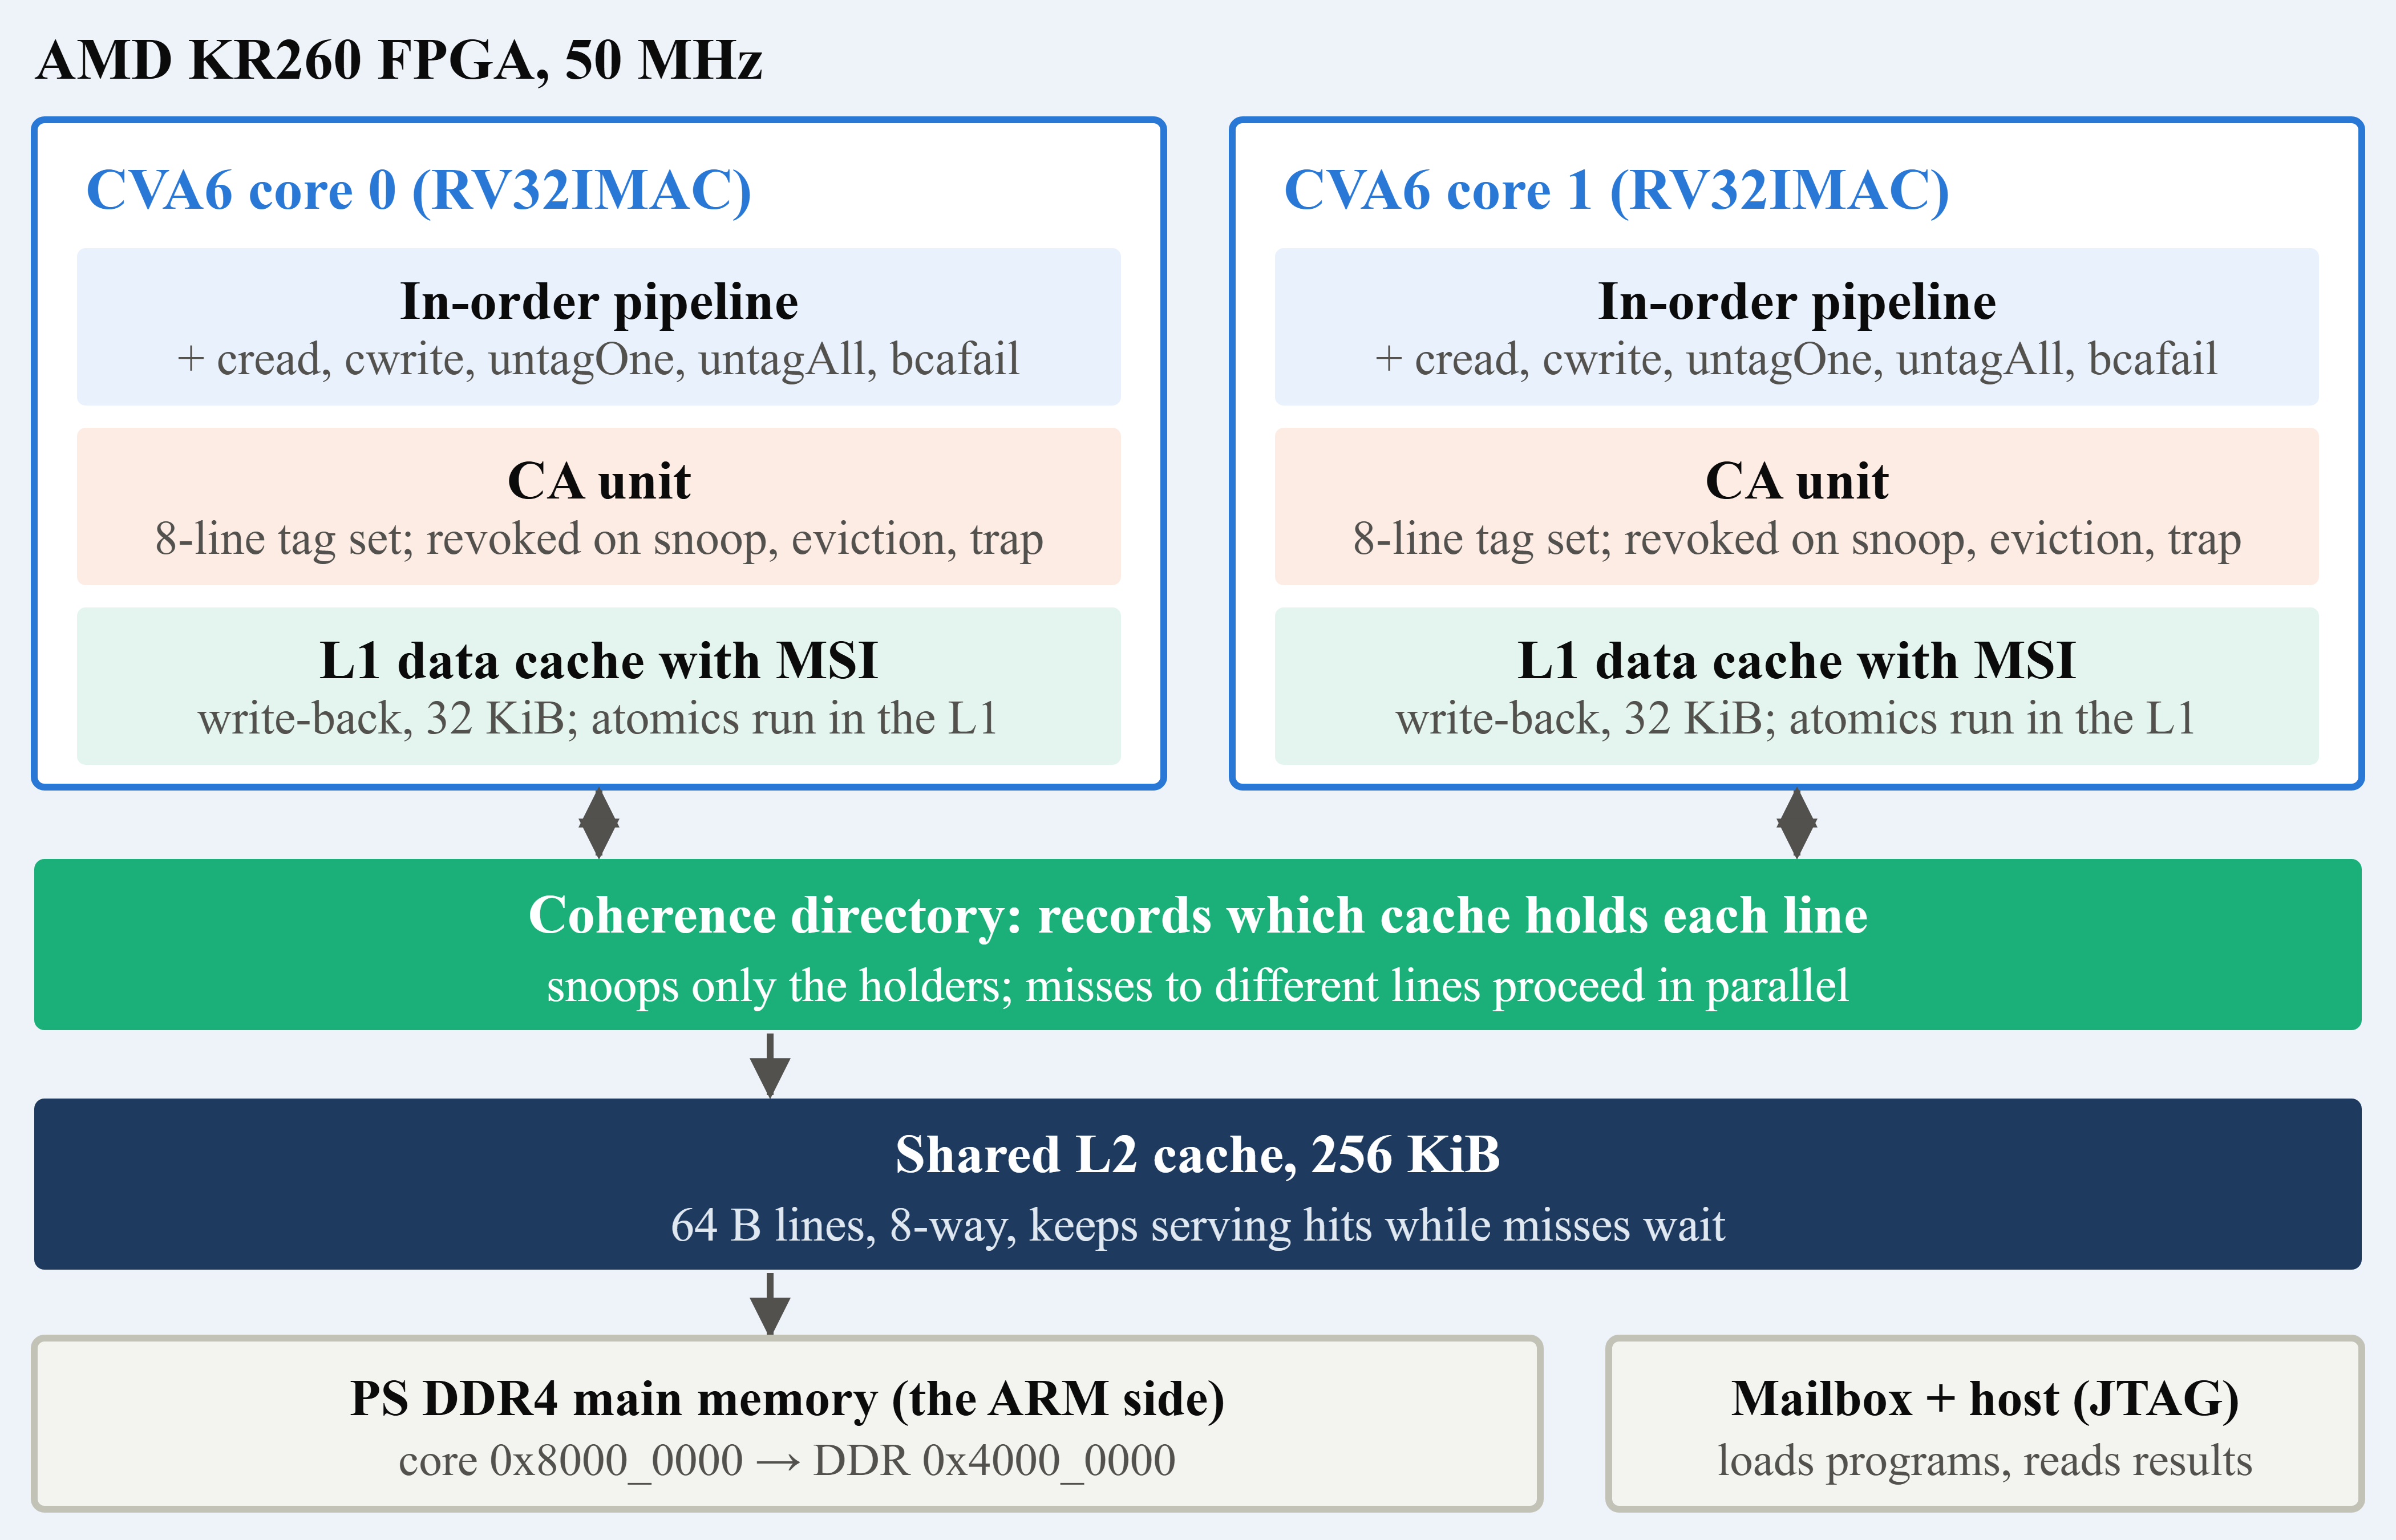
\includegraphics[width=0.97\linewidth]{architecture_v3.png}\par}
  \vspace{4pt}\stepcounter{pfig}{\fontsize{16}{20}\selectfont\color{captiongray}\textbf{Figure \thepfig.}
  Our two-core system on the AMD KR260. To CVA6 we added the coherent L1 data caches, the
  MSI directory, the CA units (with \texttt{bcafail}) and the shared L2.\par}\vspace{2pt}
\end{minipage}}\par\vspace{2pt}

\vspace{6pt}\noindent\colorbox{statbg}{\begin{minipage}{\dimexpr\columnwidth-2\fboxsep\relax}
  \vspace{4pt}{\centering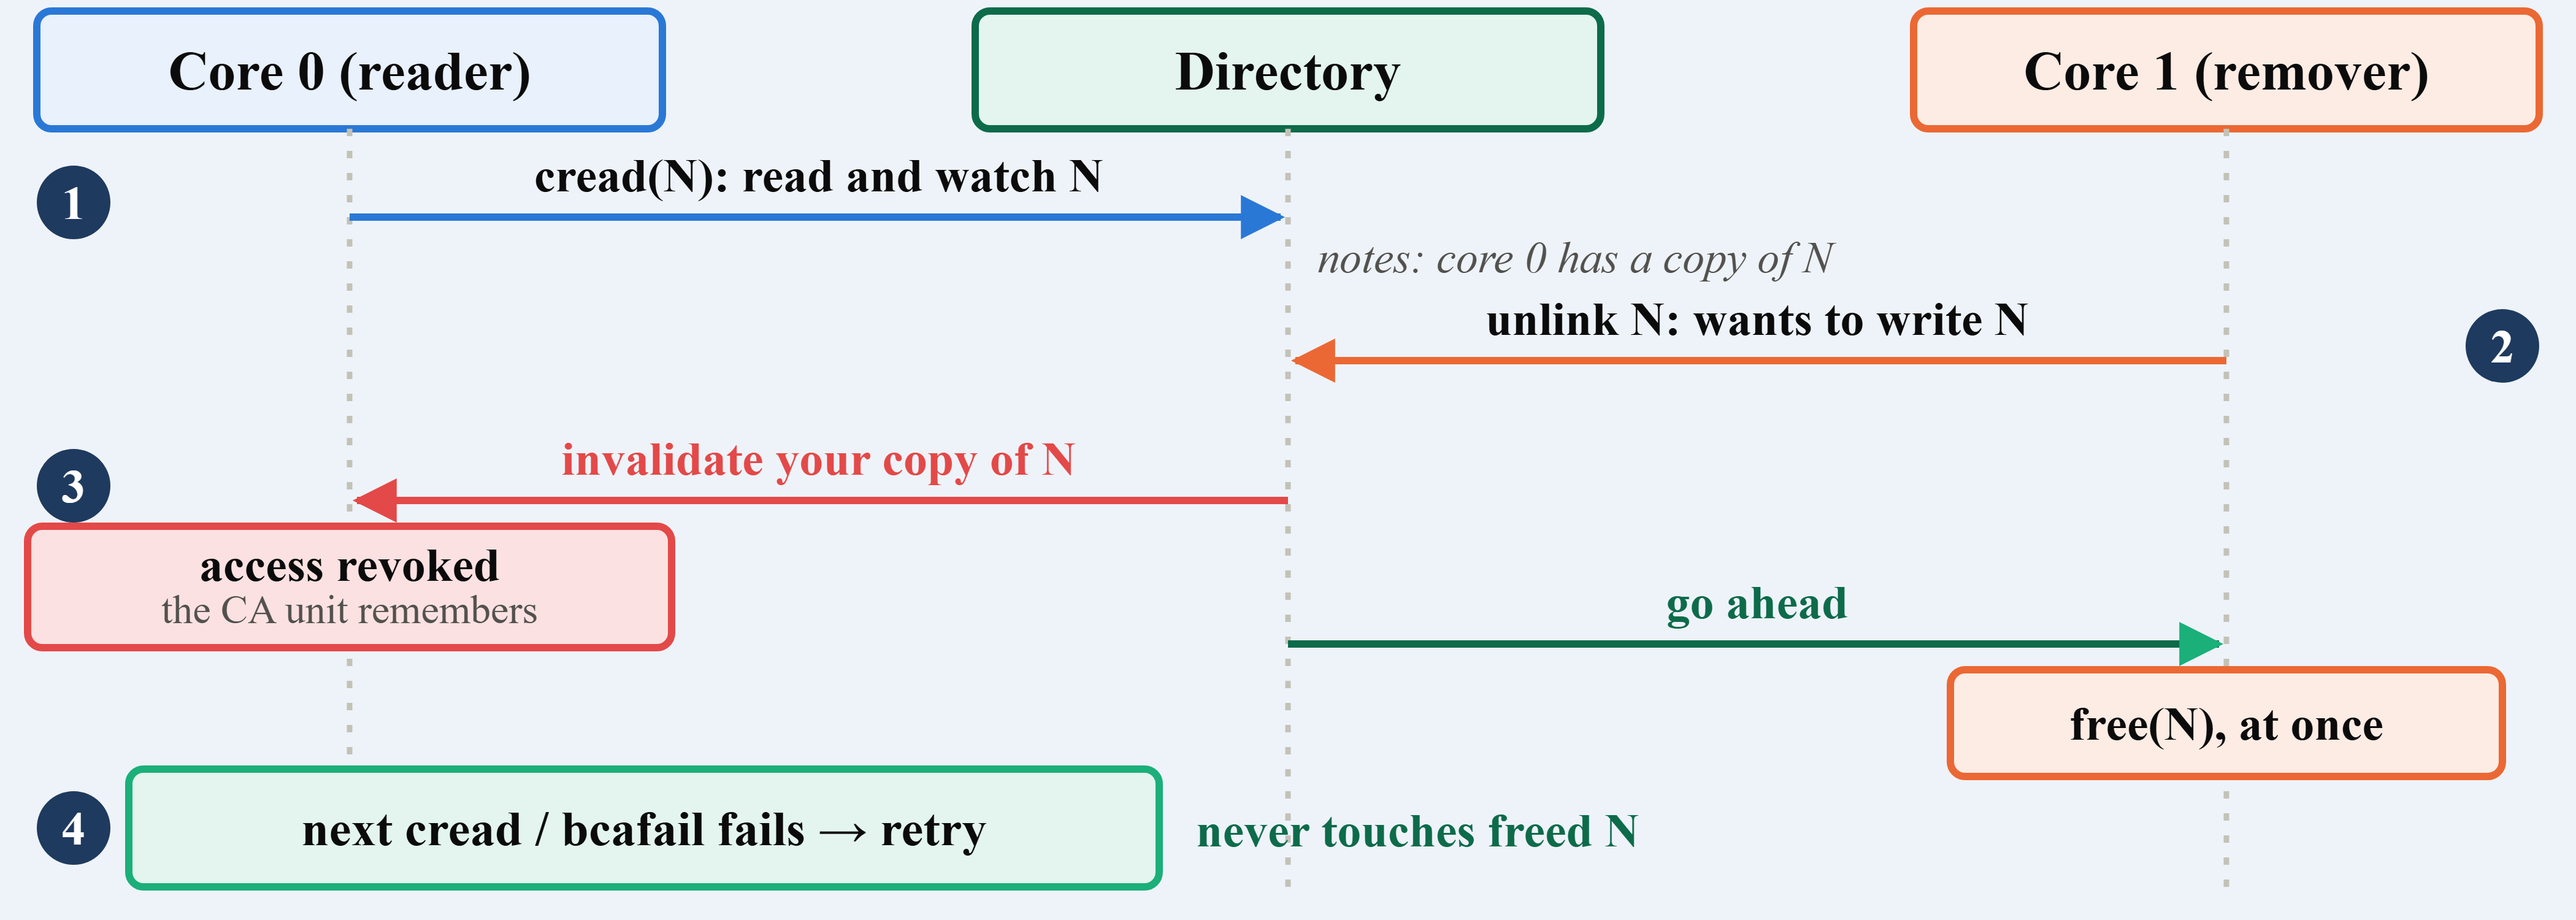
\includegraphics[width=0.84\linewidth]{revoke_seq.png}\par}
  \vspace{4pt}\stepcounter{pfig}{\fontsize{16}{20}\selectfont\color{captiongray}\textbf{Figure \thepfig.}
  CA reuses the coherence messages the caches already exchange: the remover's write
  invalidates the reader's copy, and that revokes its access.\par}\vspace{2pt}
\end{minipage}}\par



\columnbreak
%----------------------------------------------------------------------------------------
\psection{From paper to hardware: challenges and lessons}
%----------------------------------------------------------------------------------------
Turning a simulated idea into a working chip meant solving problems the paper never faced.\par
{\centering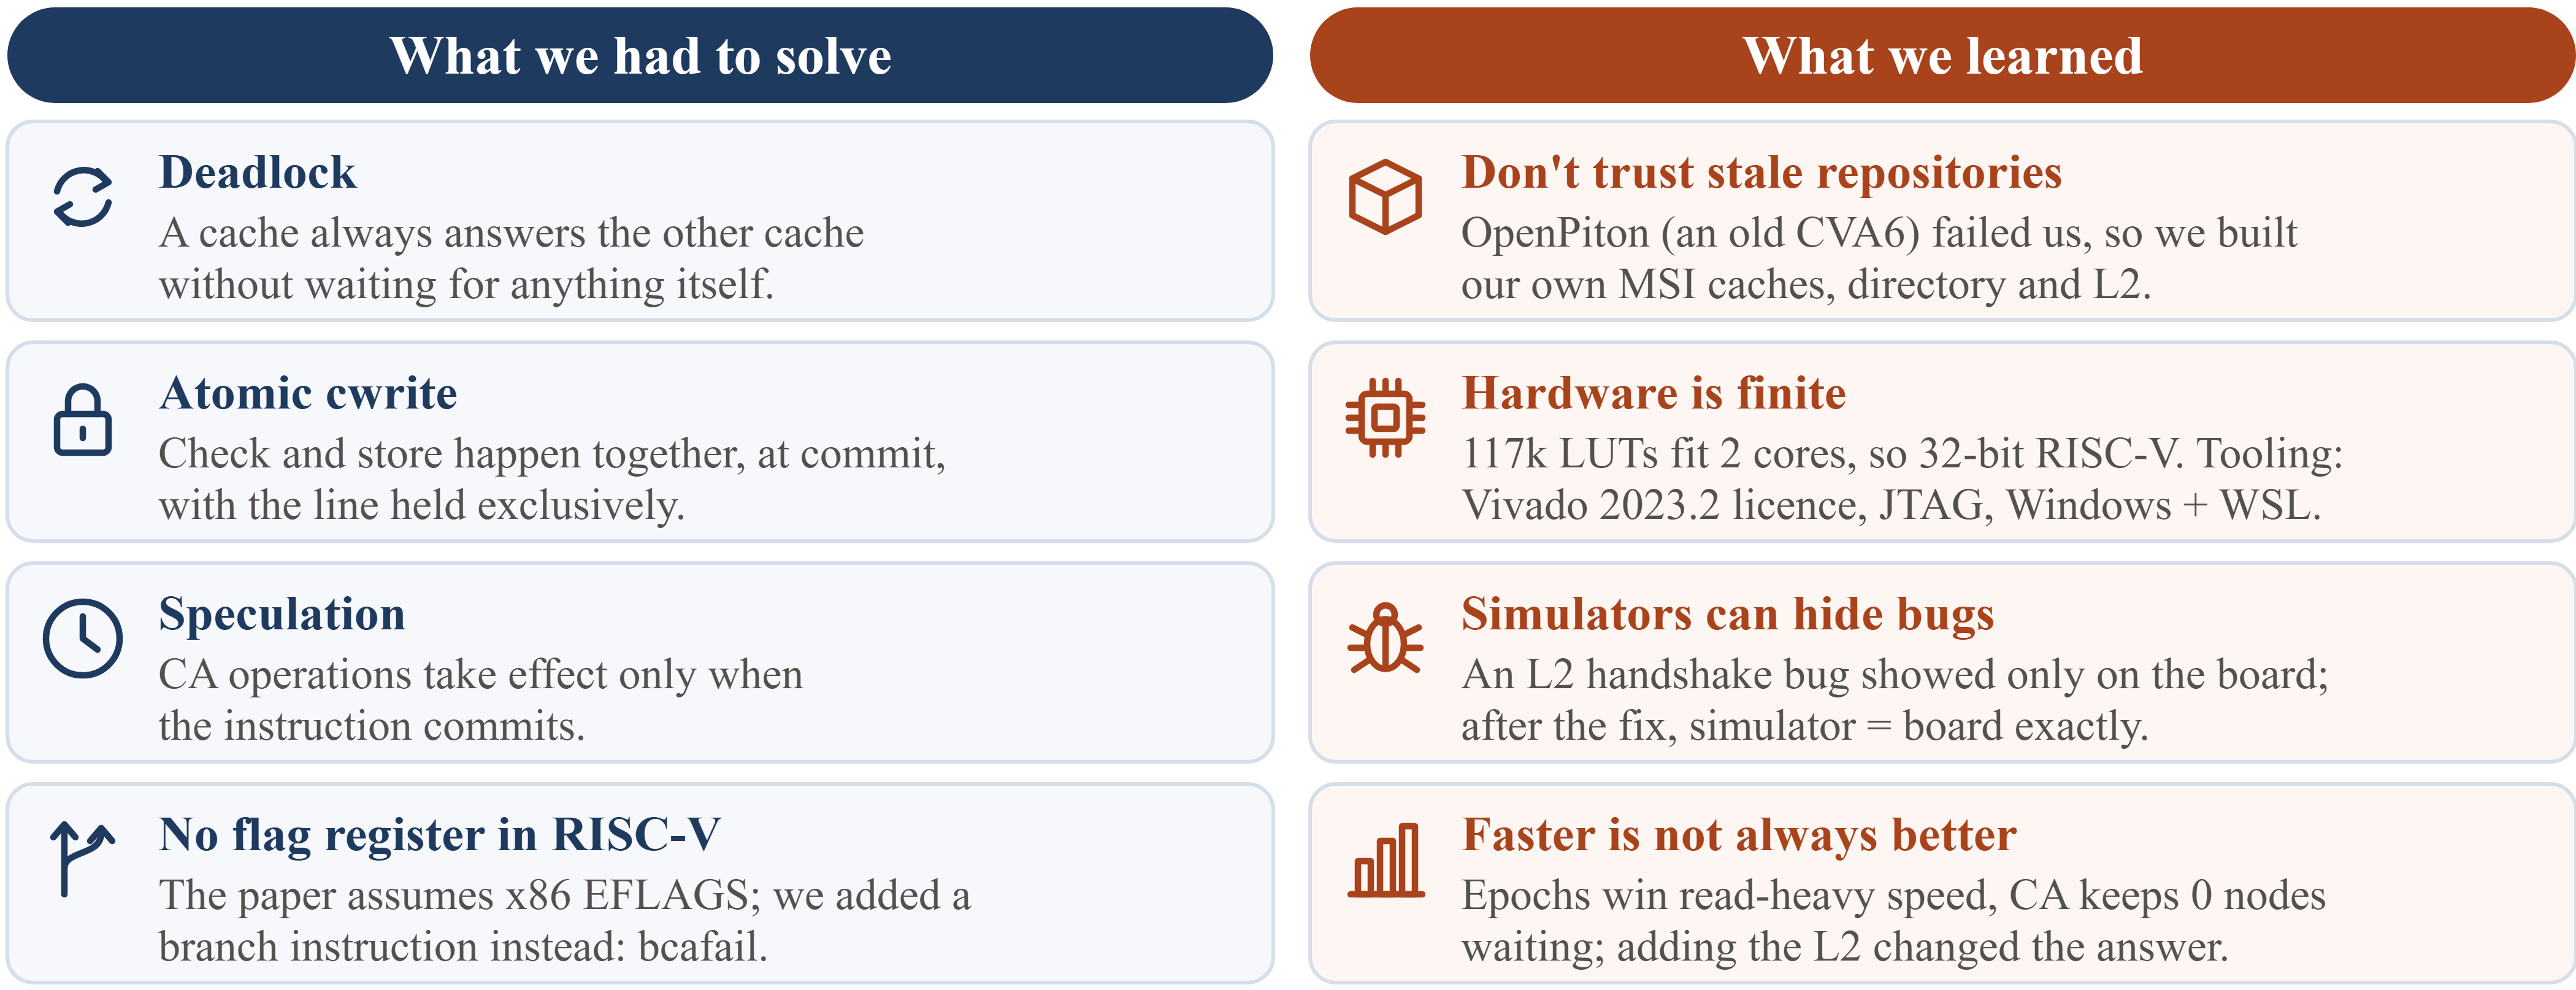
\includegraphics[width=\columnwidth]{challenges_lessons.png}\par}


%----------------------------------------------------------------------------------------
\psection{Evaluation}
%----------------------------------------------------------------------------------------
\psub{How we know it works}
{\centering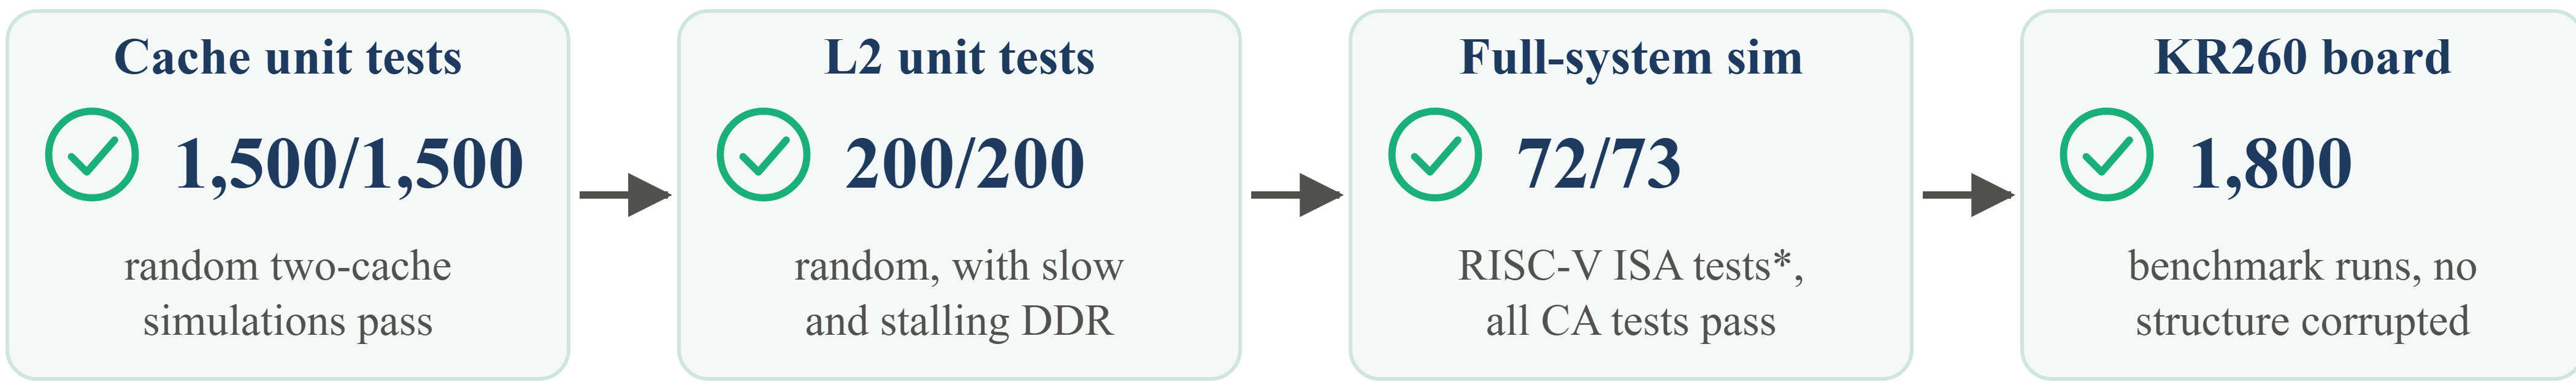
\includegraphics[width=\columnwidth]{verify_flow.png}\par}
{\smallsize 26 of 27 deliberately injected bugs are caught. Negative control: with plain
loads the board reads freed memory; with \texttt{cread} it never does.
\textsuperscript{*}The failing ISA test is also disabled upstream.\par}

\psub{Setup}
The four benchmarks of~[1] (lazy list, BST, stack, hash table) with 0\% and 100\% updates,
on two cores with 16\,B L1 lines and a shared 256\,KiB L2 (the paper: up to 32 threads, 64\,B
lines, a shared L2), on the \textbf{KR260 board} and in a \textbf{simulator of the same design}.



\psub{Results}
\posterfig[0.77]{throughput_v3.png}{Throughput on the board relative to never freeing memory
(higher is better). CA uses its best check method for each workload.}



\noindent
\begin{minipage}[t]{0.47\columnwidth}
  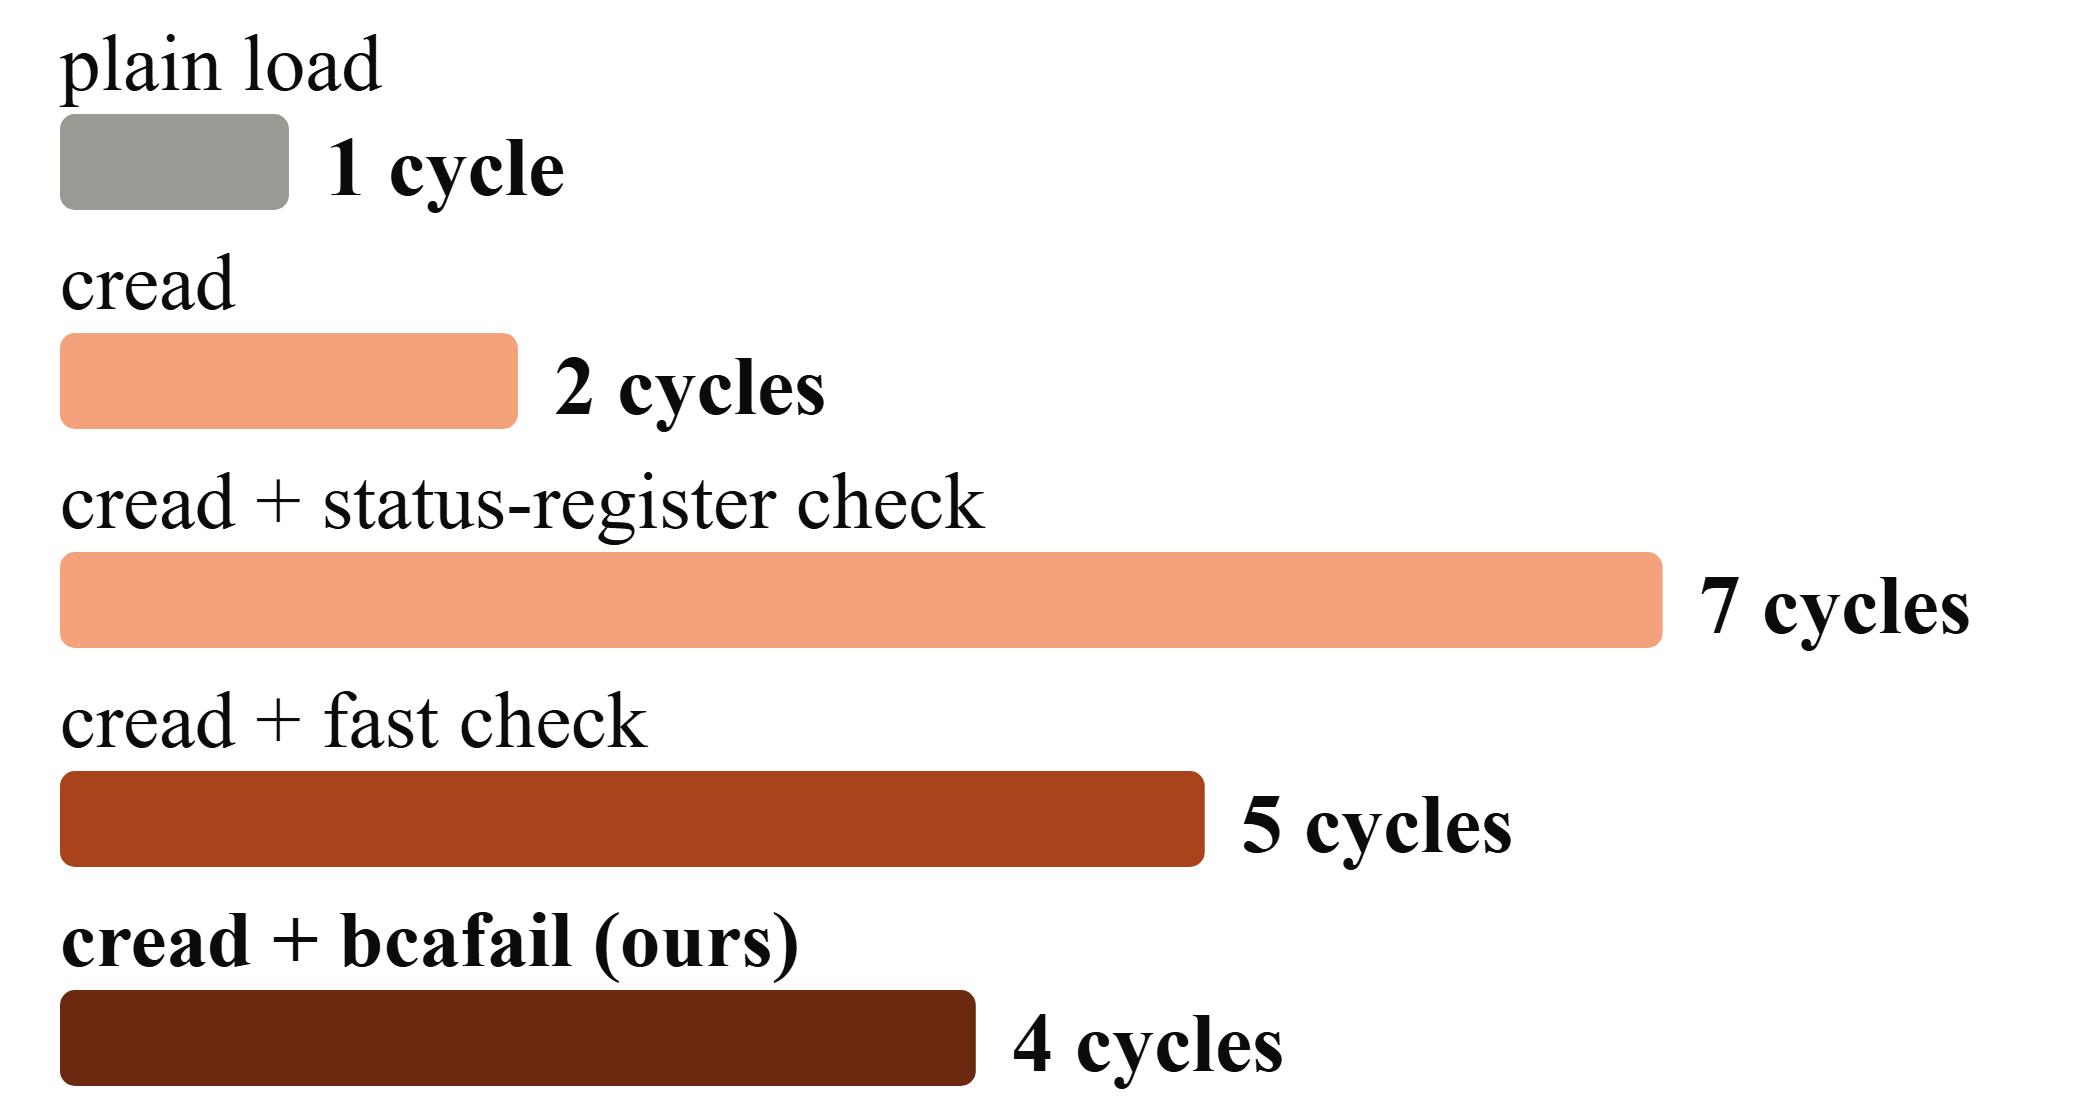
\includegraphics[width=\linewidth]{read_cost_v3.png}
  \pcaption{Cycles for one protected read.}
\end{minipage}\hfill
\begin{minipage}[t]{0.5\columnwidth}
  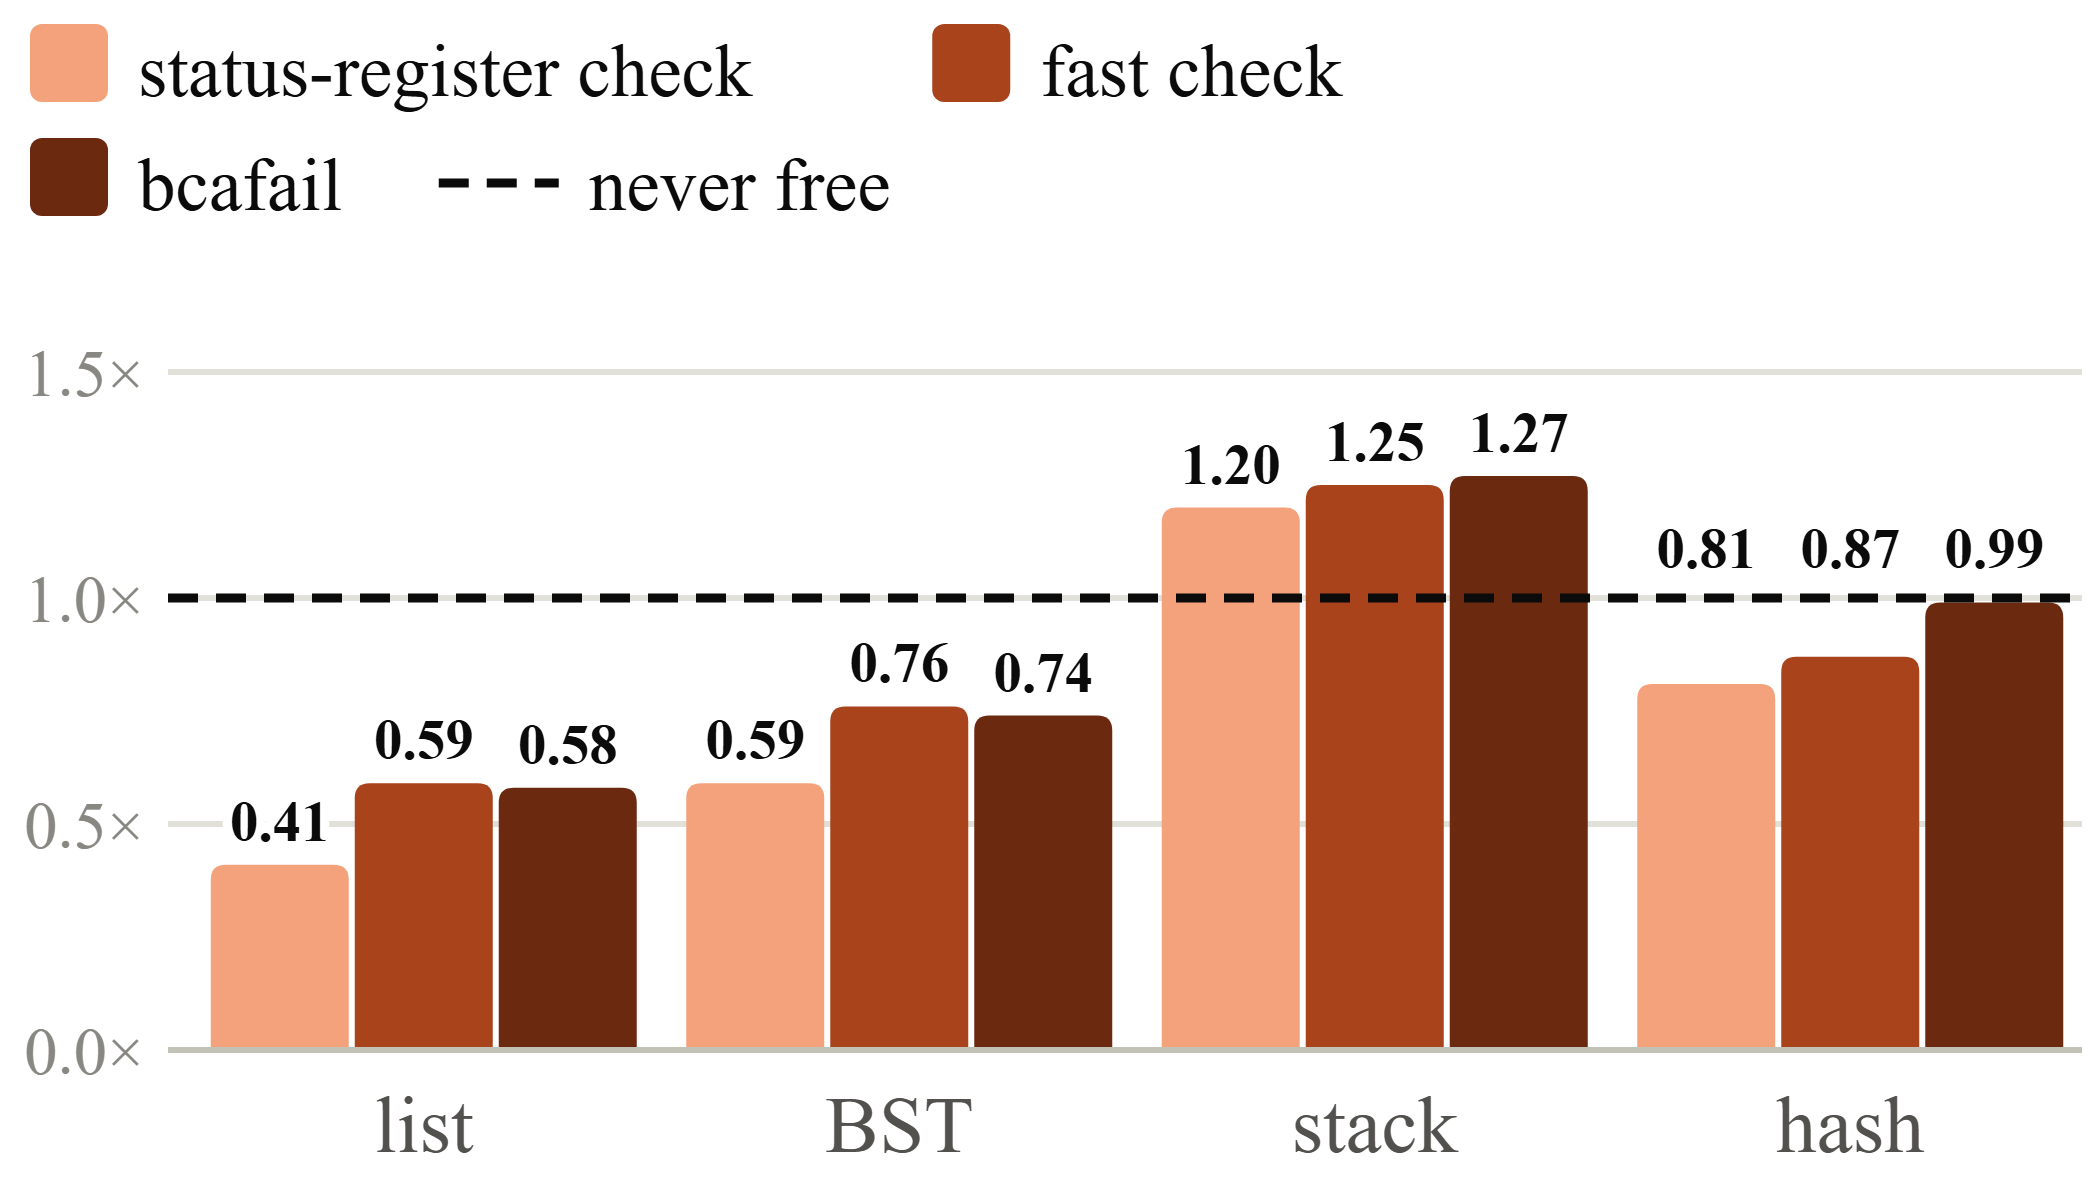
\includegraphics[width=\linewidth]{ca_variants_half.png}
  \pcaption{CA throughput by check method (board, 100\% updates, relative to never freeing).
  \texttt{bcafail} wins when failures are frequent.}
\end{minipage}

\vspace{4pt}\noindent
\begin{minipage}[t]{0.47\columnwidth}
  \vspace{0pt}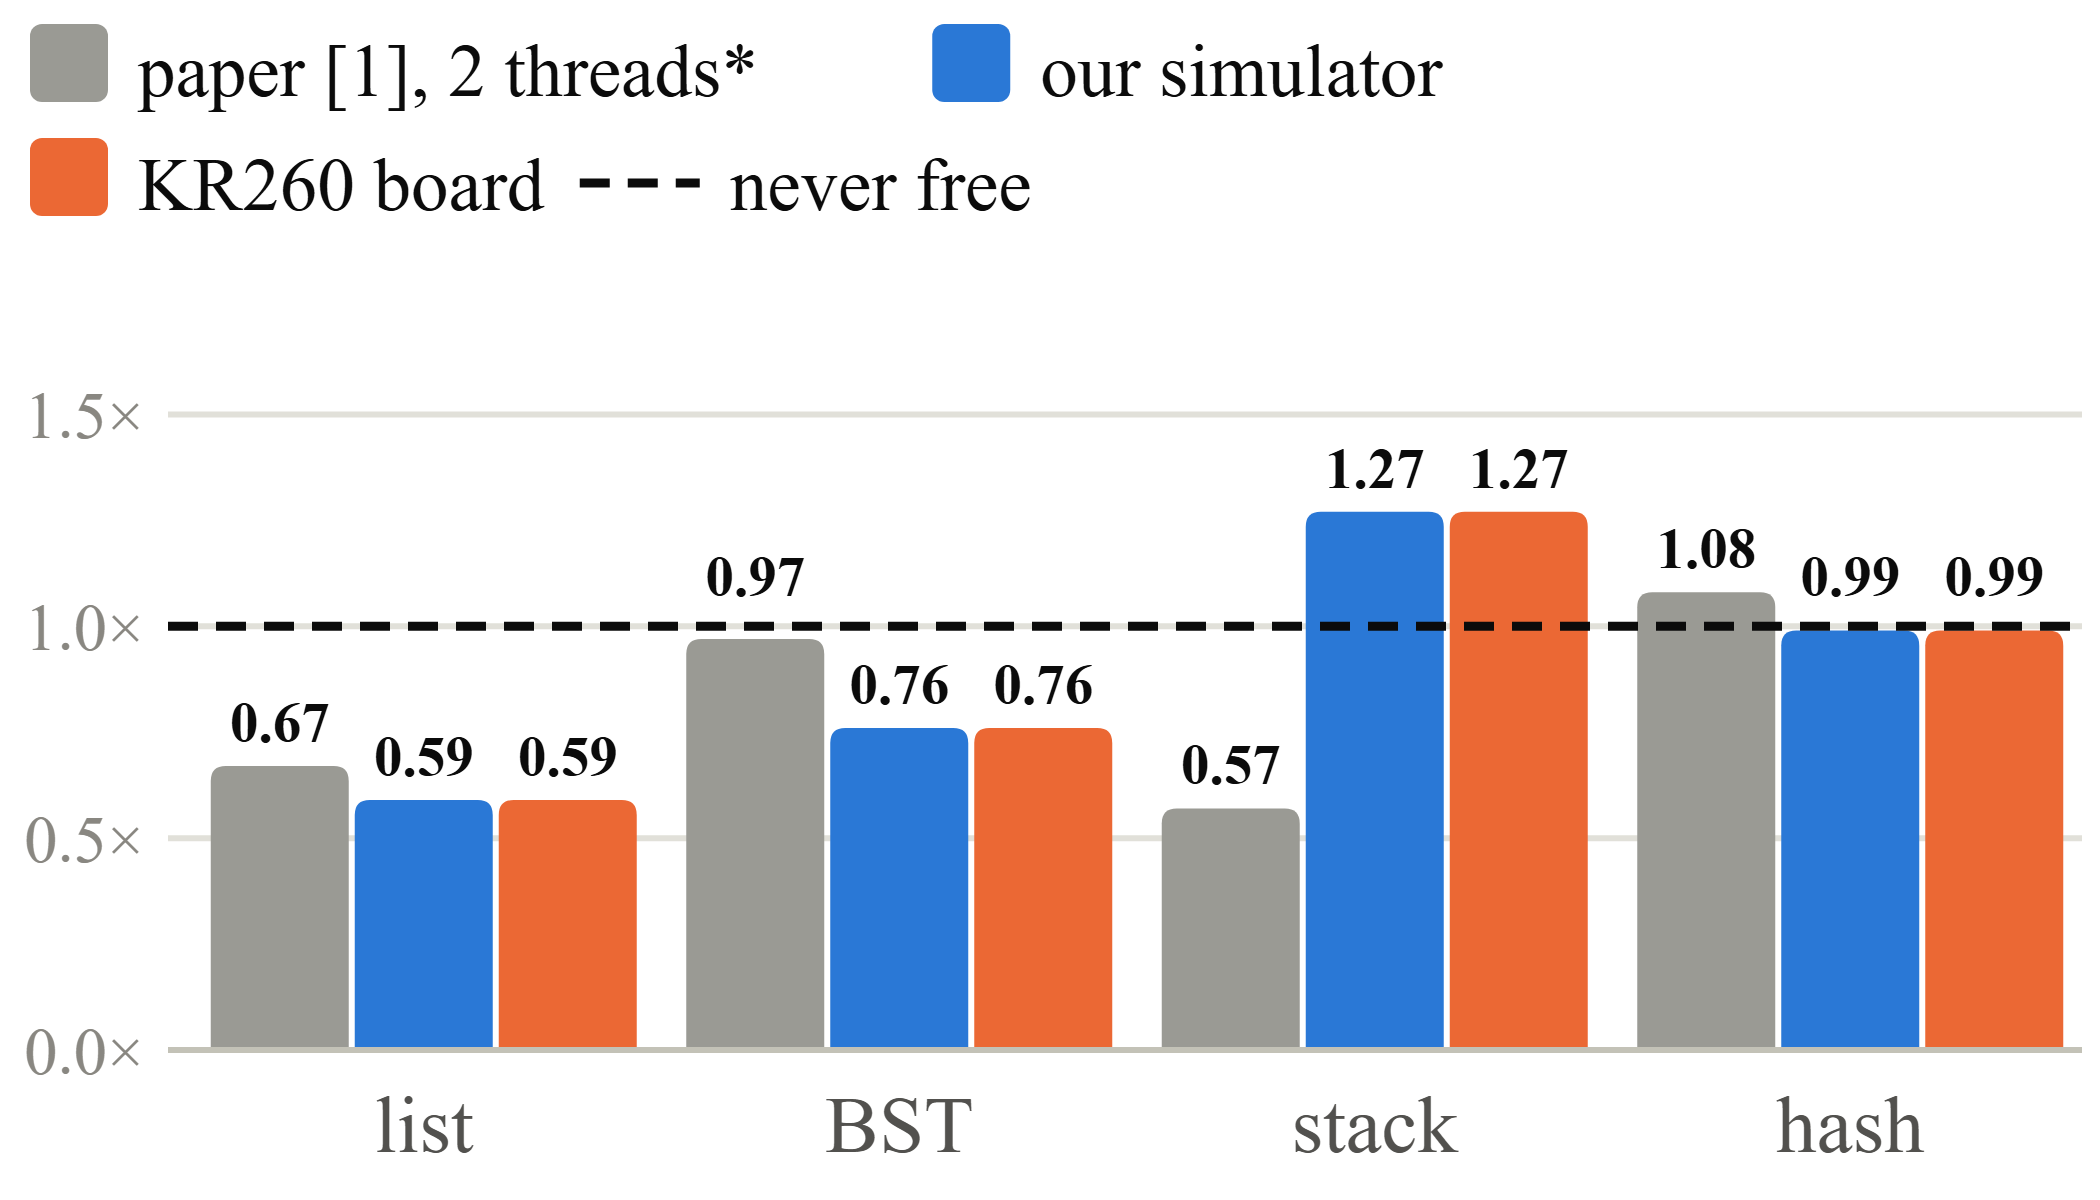
\includegraphics[width=\linewidth]{paper_sim_board_half.png}
  \pcaption{CA (ours: best check) vs.\ never freeing, 100\% updates. Our simulator and board agree exactly
  (all 144 configurations).\newline \textsuperscript{*}\mbox{Paper:} read off its plot between 1 and 4 threads.}
\end{minipage}\hfill
\begin{minipage}[t]{0.5\columnwidth}\vspace{0pt}
\begin{itemize}[leftmargin=1.2em,itemsep=6pt]
  \key{\textbf{Under contention CA is fastest:} 1.27$\times$ on the stack, 0.99 on the hash
       table, ahead of epochs (1.03, 0.91) and hazard pointers (0.99, 0.69).}
  \key{\textbf{CA frees every node at once:} 0 left waiting, against 20--34 (hazard pointers)
       and 102--202 (epochs).}
  \key{Read-heavy work: epochs are fastest on 2 cores, as in~[1] at low thread counts.}
  \key{\textbf{The shared L2} cut misses from 54 to 33 cycles and made runs up to
       2.26$\times$ faster, but also exposed CA's per-read cost.}
\end{itemize}
\end{minipage}

\vspace{6pt}\psub{Hardware cost}
{\centering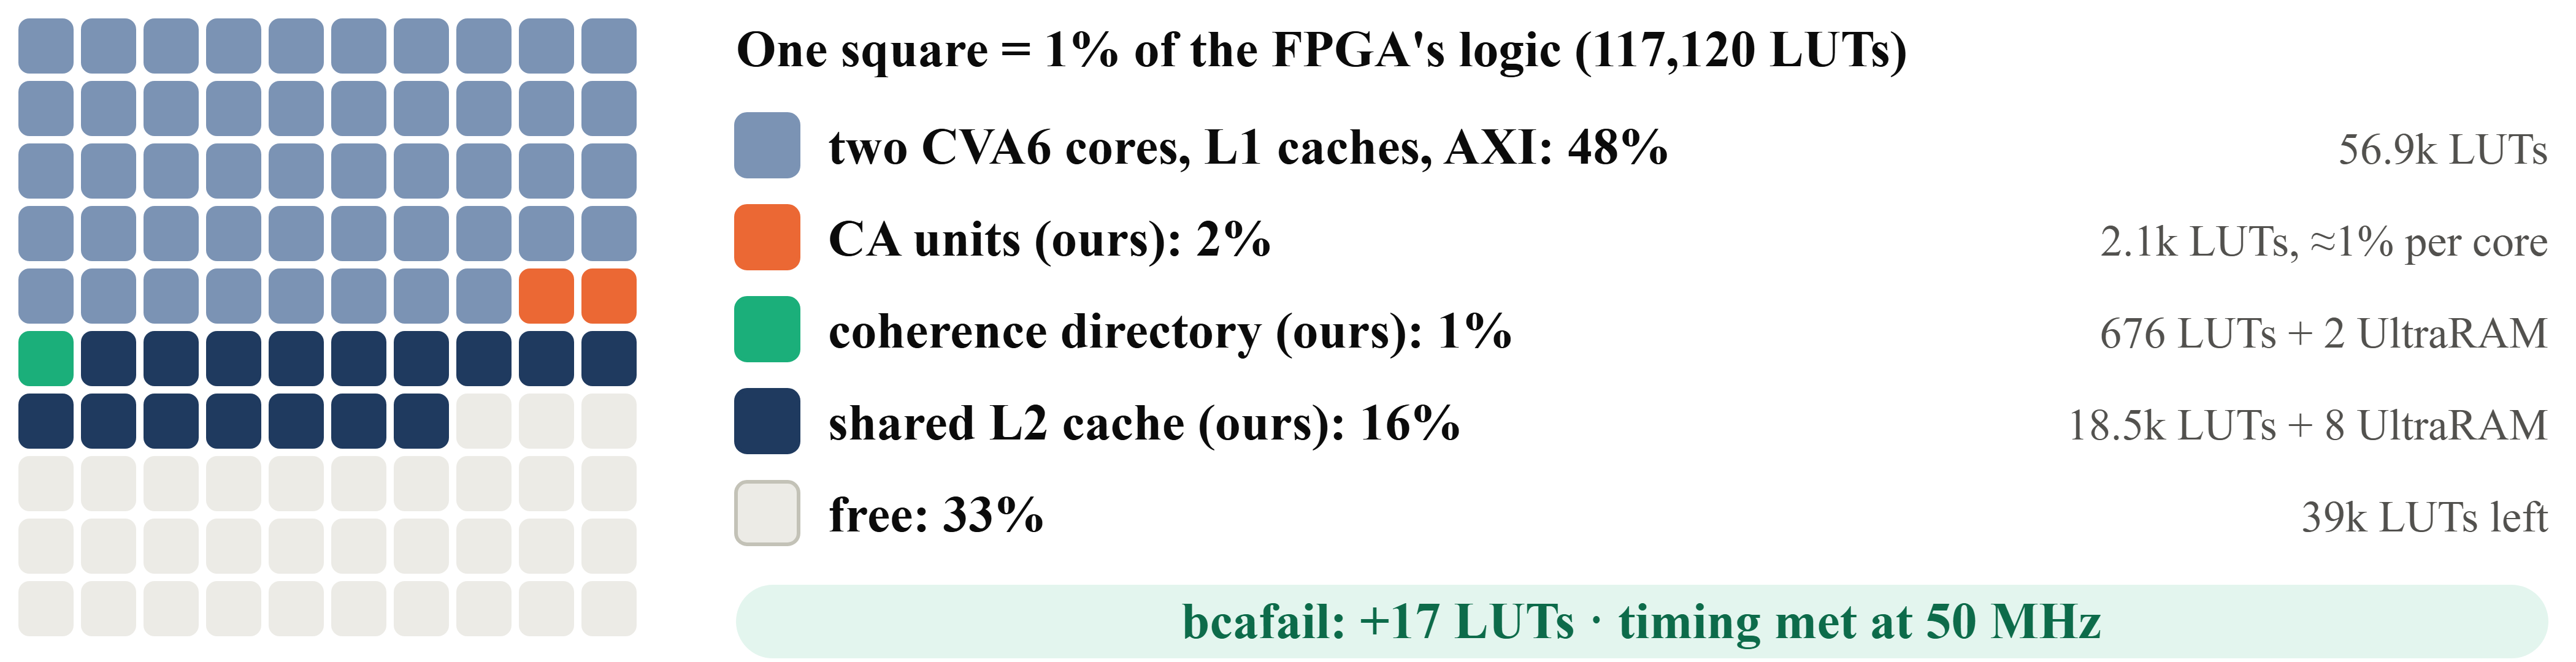
\includegraphics[width=0.8\columnwidth]{hardware_cost_v3.png}\par}

%----------------------------------------------------------------------------------------
\psection{Conclusions}
%----------------------------------------------------------------------------------------
We built a dual-core RISC-V processor with Conditional Access, directory coherence and a
shared L2 cache on an AMD KR260, and it \textbf{works on real hardware}: 1,800 benchmark runs,
no corrupted data structure. CA \textbf{frees every node immediately}, and with our
\texttt{bcafail} branch it is the \textbf{fastest scheme under contention} (1.27$\times$
never-freeing on the stack), for about 1\% of the FPGA per core. A cycle-exact simulator of the
same design matches the board exactly. Against the paper at 2 threads we are close on the list and hash table, and differ most on the stack.
\emph{Next:} more cores, to test CA where~[1] shows its largest gains.

\vspace{3pt}
{\smallsize
\textbf{Code and data:} \href{https://github.com/turing-house-community/multicore-on-fpga}{\texttt{github.com/turing-house-community/multicore-on-fpga}}\par\vspace{2pt}
\textbf{References.}
[1] A.~Singh, T.~Brown, M.~Spear. Efficient hardware primitives for immediate memory
reclamation in optimistic data structures. arXiv:2302.12958, 2023.
[2] F.~Zaruba, L.~Benini. The cost of application-class processing. \emph{IEEE TVLSI}, 2019.
[3] M.~M.~Michael. Hazard pointers. \emph{IEEE TPDS}, 2004.
[4] T.~E.~Hart et al. Performance of memory reclamation for lockless synchronization.
\emph{JPDC}, 2007.\par\vspace{3pt}
\textbf{Acknowledgements.} We thank Prof.\ Ajay Singh for his guidance, and the Department
of Computer Science and Engineering, IIT Gandhinagar, for the AMD KR260 board and tools.\par}

\end{multicols}
\end{document}
